\documentclass[12pt, a4paper] {ncc}
\usepackage[utf8] {inputenc}
\usepackage[T2A]{fontenc}
\usepackage[english, russian] {babel}
\usepackage[usenames,dvipsnames]{xcolor}
\usepackage{listings,a4wide,longtable,amsmath,amsfonts,graphicx}
\usepackage{indentfirst}
\usepackage{bytefield}
\usepackage{multirow}
\usepackage{float}
\usepackage{caption}
\usepackage{subcaption}
\captionsetup{compatibility=false}
\usepackage{tabularx}

\usepackage[left=2cm,right=2cm,top=2cm,bottom=2cm,bindingoffset=0cm]{geometry}

\begin{document}
\setcounter{figure}{0}
\frenchspacing
\pagestyle{empty}
\begin{center}
                            Университет ИТМО    \\
                        Кафедра вычислительной техники

\vspace{\stretch{2}}
			Основы теории автоматического управления
\end{center}
\vspace{\stretch{2}}
\begin{center}
			Лабораторная работа № 3 \\
    <<Построение и исследование моделей внешних воздействий>>
\end{center}
\vspace{\stretch{3}}
\begin{flushright}
                                    Студент:\\
                                    {\it Куклина М.Д., P3401}\\
                                    Преподаватель: \\
                                    {\it Кремлёв А.С.}
\end{flushright}
\vspace{\stretch{4}}
\begin{center}
                             Санкт-Петербург, 2018
\end{center}
\newpage

\section{Расчёт параметров и синтез математических моделей командных генераторов}

	\subsection{Командный генератор гармонического сигнала}

		\begin{description}
    		\item[Угол сканирования $\phi$:] 24.
    		\item[Частота сканирования$f$:]  2.
		\end{description}

		Гармоническая функция $g(t) = A\sin (\omega t)$. \\

		\[\omega = 2 \pi f \approx 12.56\]

		\[A = \dfrac {\tg \phi} {\omega} = \dfrac {0.445} {12.56} = 0.0354\]
		
		Таким образом, гармоническая функция обретает вид: $g(t) = 0.0354 \sin (12.56t)$.

		Матрица коэффициентов:
		\[G = 
			\begin{bmatrix}
				0 & 1 \\
			   -156.75 & 0
			\end{bmatrix}
			H = \begin{bmatrix}
					1 & 0
				\end{bmatrix}
		\]

		Начальные условия: $z_1(0) = 0, z_2(0) = A \omega = 0.44624$
	\subsection{Командный генератор с трапецеидальным графиком скорости}

		\begin{description}
			\item[Амплитуда скорости $\Delta$] 4.
			\item[Амплитуда ускорения $V$] 2.
			\item[Конечное значение $F$] 10.
		\end{description}

		Из исходных данных получаем значения для времён.\\
		\begin{itemize}
			\item Найдём точку $t_A$ из интегрирования ускорения.

				\[v = \int \limits_0^{t_A} \Delta \; \mathrm{d}t = \Delta \cdot t_A \implies  t_A = \dfrac {V} {\delta} = 0.5\]

			\item Найдем момент времени, когда перемещение равно F в точке $t_C$.

        		\[P(t_C) = \dfrac {\Delta} {2} t_C^2 + v \cdot t_C - F = 2 t_C^2 + 2 t_C - 10\].
				\[\text{roots} = \begin{bmatrix}
							-3.2 \\ 2.2
					\end{bmatrix}
					\implies t_C = 2.2
				\].
			
			\item Найдём момент времени $t_B$.
				\[v = \int \limits_{t_B}^{t_C} \Delta \; \mathrm{d}t 
					=  \Delta \cdot (t_C - t_B) \implies t_B 
    				= \dfrac {\Delta t_C - v} {\Delta} = 1.7
				\]

		\end{itemize}

		Матрица коэффициентов:
		\[G = 
			\begin{bmatrix}
				0 & 1 & 0 \\
				0 & 0 & 1 \\
				0 & 0 & 0
			\end{bmatrix}
			H = \begin{bmatrix}
					1 & 0 & 0
				\end{bmatrix}
		\]
		
	\subsection{Командный генератор возмущения}

		\[g(t) = 3 e^{-0.5t}\sin t + 0.2 t\]


	Воспользуемся методом последовательного дифференцирования. Будем дифференцировать до тех
	пор, пока очередная функция не окажется линейной комбинацией предыдущих.\\
		$g(t) = z_1$ \\
		$g^{(1)}(t) = z_2 = z^{(1)}_1 = 3  e^{-0.5t} \cos t - 1.5 e^{-0.5t} \sin t + 0.2$ \\
		$g^{(2)}(t) = z_3 = z^{(1)}_2 = -3e^{-0.5t}\cos t - 2.25e^{-0.5t}\sin t$ \\
		$g^{(3)}(t) = z_4 = z^{(1)}_3 = -0.75e^{-0.5t}\cos t + 4.125e^{-0.5t}\sin t$ \\
		$g^{(4)}(t) = z^{(1)}_4 = 4.5e^{-0.5t}\cos t - 1.3125e^{-0.5t}\sin t$ \\
		$g^{(5)}(t) = Ag^{(2)} + Bg^{(3)} $ \\

	\[
		\begin{cases}
			4.5 = -3 A - 0.75 B\\
			-1.3125 = -2.25 A + 4.125 B\\
		\end{cases}
		\implies
		A = -1.25, B = -1
	\]


		Матрица коэффициентов:
		\[
			Z = \begin{bmatrix}
				z_1 \\ z_2 \\ z_3 \\ z_4
			\end{bmatrix}
			G = 
			\begin{bmatrix}
				0 & 1 & 0 & 0\\
				0 & 0 & 1 & 0 \\
				0 & 0 & 0 & 1 \\
				0 & -1.25 & -1 & 0
			\end{bmatrix}
			H = \begin{bmatrix}
					1 & 0 & 0
				\end{bmatrix}
		\]

		Начальные условия интеграторов:\\
		$z_1(0) = 0$
		$z_2(0) = 3.2$
		$z_3(0) = -3$
		$z_4(0) = -0.75$

\section{Схемы моделирования командных генераторов}
	Схемы на рисунках 1-3.

	\begin{figure}[ht!]
		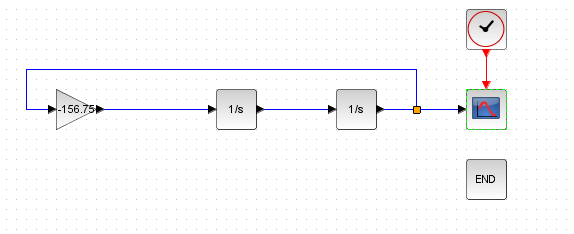
\includegraphics[scale=0.5]{./model_sin.png}
		\caption{Модель командного генератора синусоидального сигнала.}
	\end{figure}

	\begin{figure}[ht!]
		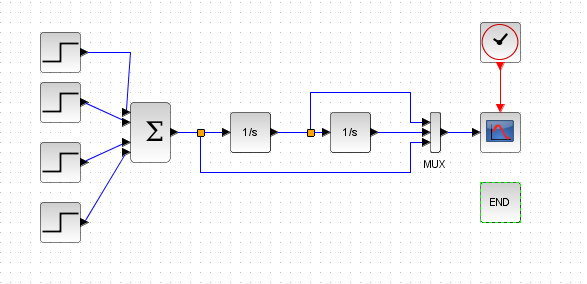
\includegraphics[scale=0.5]{./model_trap.png}
		\caption{Модель командного генератора cигнала с трапецеидальным графиком.}
	\end{figure}

	\begin{figure}[ht!]
		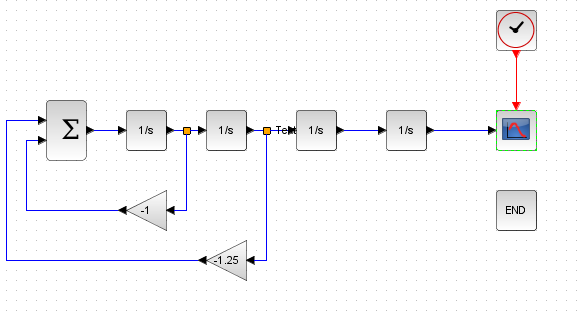
\includegraphics[scale=0.5]{./model_v.png}
		\caption{Модель командного генератора возмущения.}
	\end{figure}

\section{Результаты моделирования}

	Результаты на рисунках 4-7.
	\begin{figure}[ht!]
		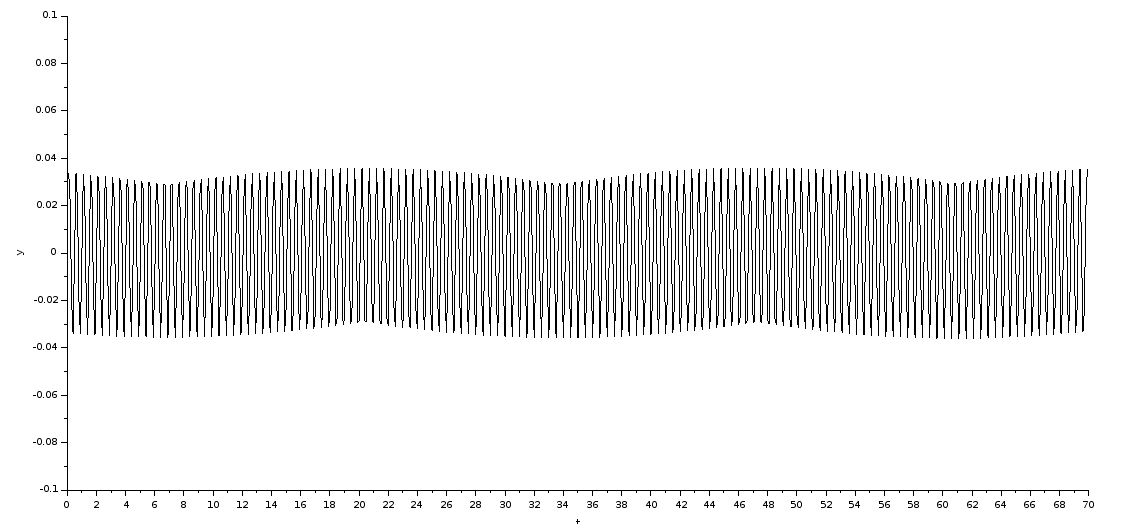
\includegraphics[scale=0.4]{./plot_sin.png}
		\caption{График командного генератора синусоидального сигнала.}
	\end{figure}
	\begin{figure}[ht!]
		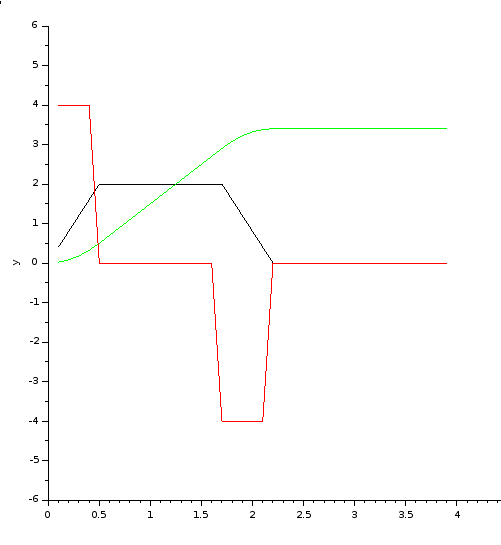
\includegraphics[scale=0.5]{./plot_trap.png}
		\caption{График командного генератора cигнала с трапецеидальным графиком.}
	\end{figure}

	\begin{figure}[ht!]
		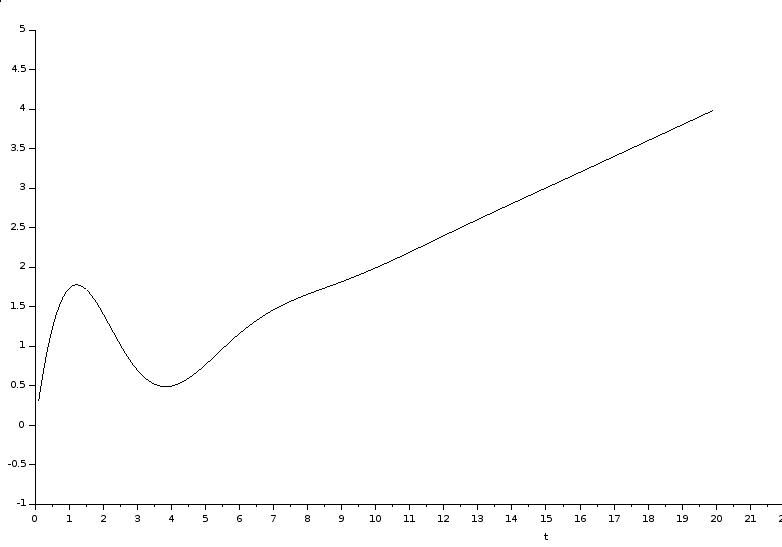
\includegraphics[scale=0.5]{./plot_v.png}
		\caption{График командного генератора возмущения.}
	\end{figure}
\section{Выводы}

В результате выполнения лабораторной работы произошло ознакомление
с принципами построения моделей внешних воздействий и с методом
последовательного дифференцирования. В ходе выполнения работы
возникли трудности в силу недостаточного количества информации
в описании лабораторной и отсутствия ссылок на вспомогательную
литературу.

\end{document}
